\documentclass{standalone}
\usepackage{tikz}
\usetikzlibrary{patterns, positioning}


\begin{document}
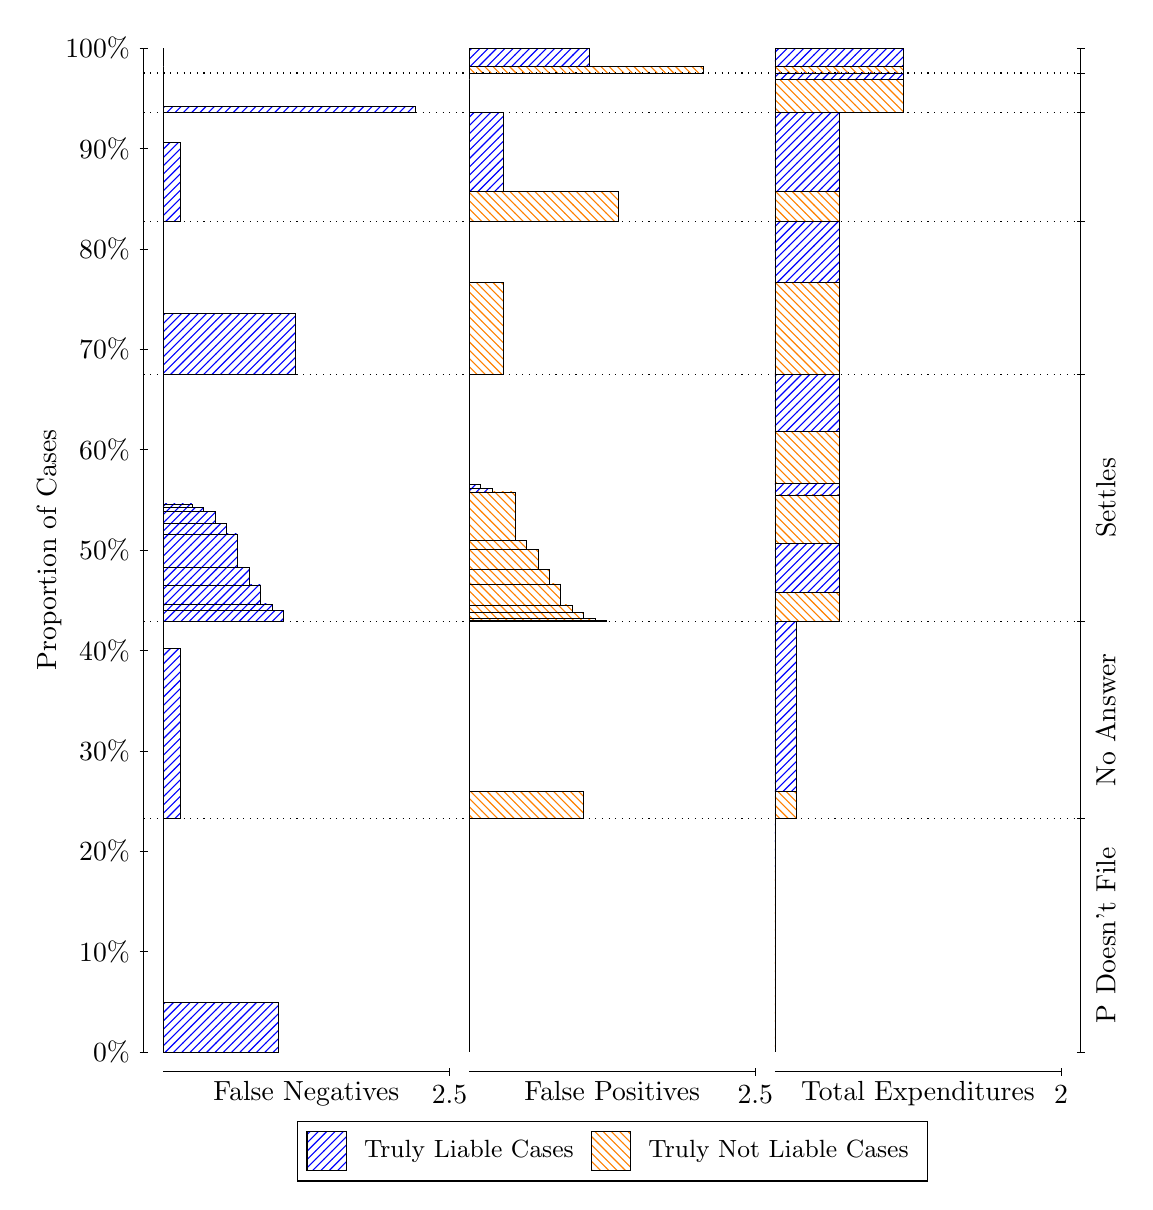
\begin{tikzpicture}
\draw[black, very thin] (1.5,1.75) -- (1.5,14.5);
\node[rotate=90, text=black, anchor=center] at (0.3, 8.125) {Proportion of Cases};
\draw[black, very thin] (1.45,1.75) -- (1.55,1.75);
\node[text=black, anchor=east] at (1.45, 1.75) {0\%};
\draw[black, very thin] (1.45,3.025) -- (1.55,3.025);
\node[text=black, anchor=east] at (1.45, 3.025) {10\%};
\draw[black, very thin] (1.45,4.3) -- (1.55,4.3);
\node[text=black, anchor=east] at (1.45, 4.3) {20\%};
\draw[black, very thin] (1.45,5.575) -- (1.55,5.575);
\node[text=black, anchor=east] at (1.45, 5.575) {30\%};
\draw[black, very thin] (1.45,6.85) -- (1.55,6.85);
\node[text=black, anchor=east] at (1.45, 6.85) {40\%};
\draw[black, very thin] (1.45,8.125) -- (1.55,8.125);
\node[text=black, anchor=east] at (1.45, 8.125) {50\%};
\draw[black, very thin] (1.45,9.4) -- (1.55,9.4);
\node[text=black, anchor=east] at (1.45, 9.4) {60\%};
\draw[black, very thin] (1.45,10.675) -- (1.55,10.675);
\node[text=black, anchor=east] at (1.45, 10.675) {70\%};
\draw[black, very thin] (1.45,11.95) -- (1.55,11.95);
\node[text=black, anchor=east] at (1.45, 11.95) {80\%};
\draw[black, very thin] (1.45,13.225) -- (1.55,13.225);
\node[text=black, anchor=east] at (1.45, 13.225) {90\%};
\draw[black, very thin] (1.45,14.5) -- (1.55,14.5);
\node[text=black, anchor=east] at (1.45, 14.5) {100\%};

\draw[black, very thin] (13.4,1.75) -- (13.4,14.5);
\draw[black, very thin] (13.35,1.75) -- (13.45,1.75);
\node[anchor=west] at (13.35, 1.75) {};
\draw[black, very thin] (13.35,4.7179) -- (13.45,4.7179);
\node[anchor=west] at (13.35, 4.7179) {};
\draw[black, very thin] (13.35,7.2155) -- (13.45,7.2155);
\node[anchor=west] at (13.35, 7.2155) {};
\draw[black, very thin] (13.35,10.358) -- (13.45,10.358);
\node[anchor=west] at (13.35, 10.358) {};
\draw[black, very thin] (13.35,12.301) -- (13.45,12.301);
\node[anchor=west] at (13.35, 12.301) {};
\draw[black, very thin] (13.35,13.681) -- (13.45,13.681);
\node[anchor=west] at (13.35, 13.681) {};
\draw[black, very thin] (13.35,14.183) -- (13.45,14.183);
\node[anchor=west] at (13.35, 14.183) {};
\draw[black, very thin] (13.35,14.5) -- (13.45,14.5);
\node[anchor=west] at (13.35, 14.5) {};

\draw[black, very thin, pattern color=blue, pattern=north east lines] (1.75,1.75) rectangle (3.2033,2.3828);
\draw[black, very thin, pattern color=orange, pattern=north west lines] (1.75,2.3828) rectangle (1.75,4.7179);
\draw[black, very thin, pattern color=blue, pattern=north east lines] (1.75,4.7179) rectangle (1.968,6.8717);
\draw[black, very thin, pattern color=orange, pattern=north west lines] (1.75,6.8717) rectangle (1.75,7.2155);
\draw[black, very thin, pattern color=blue, pattern=north east lines] (1.75,7.2155) rectangle (3.276,7.3629);
\draw[black, very thin, pattern color=blue, pattern=north east lines] (1.75,7.3629) rectangle (3.1307,7.4393);
\draw[black, very thin, pattern color=blue, pattern=north east lines] (1.75,7.4393) rectangle (2.9853,7.6828);
\draw[black, very thin, pattern color=blue, pattern=north east lines] (1.75,7.6828) rectangle (2.84,7.9066);
\draw[black, very thin, pattern color=blue, pattern=north east lines] (1.75,7.9066) rectangle (2.6947,8.3301);
\draw[black, very thin, pattern color=blue, pattern=north east lines] (1.75,8.3301) rectangle (2.5493,8.465);
\draw[black, very thin, pattern color=blue, pattern=north east lines] (1.75,8.465) rectangle (2.404,8.6125);
\draw[black, very thin, pattern color=blue, pattern=north east lines] (1.75,8.6125) rectangle (2.2587,8.6663);
\draw[black, very thin, pattern color=blue, pattern=north east lines] (1.75,8.6663) rectangle (2.1133,8.7095);
\draw[black, very thin, pattern color=orange, pattern=north west lines] (1.75,8.7095) rectangle (1.75,10.358);
\draw[black, very thin, pattern color=blue, pattern=north east lines] (1.75,10.358) rectangle (3.4213,11.13);
\draw[black, very thin, pattern color=orange, pattern=north west lines] (1.75,11.13) rectangle (1.75,12.301);
\draw[black, very thin, pattern color=blue, pattern=north east lines] (1.75,12.301) rectangle (1.968,13.305);
\draw[black, very thin, pattern color=orange, pattern=north west lines] (1.75,13.305) rectangle (1.75,13.681);
\draw[black, very thin, pattern color=blue, pattern=north east lines] (1.75,13.681) rectangle (4.9473,13.763);
\draw[black, very thin, pattern color=orange, pattern=north west lines] (1.75,13.763) rectangle (1.75,14.183);
\draw[black, very thin, pattern color=orange, pattern=north west lines] (1.75,14.183) rectangle (1.75,14.264);
\draw[black, very thin, pattern color=blue, pattern=north east lines] (1.75,14.264) rectangle (1.75,14.5);
\draw[black, very thin, pattern color=orange, pattern=north west lines] (5.6333,1.75) rectangle (5.6333,4.0851);
\draw[black, very thin, pattern color=blue, pattern=north east lines] (5.6333,4.0851) rectangle (5.6333,4.7179);
\draw[black, very thin, pattern color=orange, pattern=north west lines] (5.6333,4.7179) rectangle (7.0867,5.0616);
\draw[black, very thin, pattern color=blue, pattern=north east lines] (5.6333,5.0616) rectangle (5.6333,7.2155);
\draw[black, very thin, pattern color=orange, pattern=north west lines] (5.6333,7.2155) rectangle (7.3773,7.236);
\draw[black, very thin, pattern color=orange, pattern=north west lines] (5.6333,7.236) rectangle (7.232,7.2613);
\draw[black, very thin, pattern color=orange, pattern=north west lines] (5.6333,7.2613) rectangle (7.0867,7.3365);
\draw[black, very thin, pattern color=orange, pattern=north west lines] (5.6333,7.3365) rectangle (6.9413,7.4275);
\draw[black, very thin, pattern color=orange, pattern=north west lines] (5.6333,7.4275) rectangle (6.796,7.6948);
\draw[black, very thin, pattern color=orange, pattern=north west lines] (5.6333,7.6948) rectangle (6.6507,7.8801);
\draw[black, very thin, pattern color=orange, pattern=north west lines] (5.6333,7.8801) rectangle (6.5053,8.1302);
\draw[black, very thin, pattern color=orange, pattern=north west lines] (5.6333,8.1302) rectangle (6.36,8.2465);
\draw[black, very thin, pattern color=orange, pattern=north west lines] (5.6333,8.2465) rectangle (6.2147,8.8635);
\draw[black, very thin, pattern color=blue, pattern=north east lines] (5.6333,8.8635) rectangle (5.924,8.9067);
\draw[black, very thin, pattern color=blue, pattern=north east lines] (5.6333,8.9067) rectangle (5.7787,8.9605);
\draw[black, very thin, pattern color=blue, pattern=north east lines] (5.6333,8.9605) rectangle (5.6333,10.358);
\draw[black, very thin, pattern color=orange, pattern=north west lines] (5.6333,10.358) rectangle (6.0693,11.528);
\draw[black, very thin, pattern color=blue, pattern=north east lines] (5.6333,11.528) rectangle (5.6333,12.301);
\draw[black, very thin, pattern color=orange, pattern=north west lines] (5.6333,12.301) rectangle (7.5227,12.677);
\draw[black, very thin, pattern color=blue, pattern=north east lines] (5.6333,12.677) rectangle (6.0693,13.681);
\draw[black, very thin, pattern color=orange, pattern=north west lines] (5.6333,13.681) rectangle (5.6333,14.101);
\draw[black, very thin, pattern color=blue, pattern=north east lines] (5.6333,14.101) rectangle (5.6333,14.183);
\draw[black, very thin, pattern color=orange, pattern=north west lines] (5.6333,14.183) rectangle (8.6127,14.264);
\draw[black, very thin, pattern color=blue, pattern=north east lines] (5.6333,14.264) rectangle (7.1593,14.5);
\draw[black, very thin, pattern color=orange, pattern=north west lines] (9.5167,1.75) rectangle (9.5167,4.0851);
\draw[black, very thin, pattern color=blue, pattern=north east lines] (9.5167,4.0851) rectangle (9.5167,4.7179);
\draw[black, very thin, pattern color=orange, pattern=north west lines] (9.5167,4.7179) rectangle (9.7892,5.0616);
\draw[black, very thin, pattern color=blue, pattern=north east lines] (9.5167,5.0616) rectangle (9.7892,7.2155);
\draw[black, very thin, pattern color=orange, pattern=north west lines] (9.5167,7.2155) rectangle (10.334,7.5833);
\draw[black, very thin, pattern color=blue, pattern=north east lines] (9.5167,7.5833) rectangle (10.334,8.2081);
\draw[black, very thin, pattern color=orange, pattern=north west lines] (9.5167,8.2081) rectangle (10.334,8.8251);
\draw[black, very thin, pattern color=blue, pattern=north east lines] (9.5167,8.8251) rectangle (10.334,8.9725);
\draw[black, very thin, pattern color=orange, pattern=north west lines] (9.5167,8.9725) rectangle (10.334,9.6357);
\draw[black, very thin, pattern color=blue, pattern=north east lines] (9.5167,9.6357) rectangle (10.334,10.358);
\draw[black, very thin, pattern color=orange, pattern=north west lines] (9.5167,10.358) rectangle (10.334,11.528);
\draw[black, very thin, pattern color=blue, pattern=north east lines] (9.5167,11.528) rectangle (10.334,12.301);
\draw[black, very thin, pattern color=orange, pattern=north west lines] (9.5167,12.301) rectangle (10.334,12.677);
\draw[black, very thin, pattern color=blue, pattern=north east lines] (9.5167,12.677) rectangle (10.334,13.681);
\draw[black, very thin, pattern color=orange, pattern=north west lines] (9.5167,13.681) rectangle (11.152,14.101);
\draw[black, very thin, pattern color=blue, pattern=north east lines] (9.5167,14.101) rectangle (11.152,14.183);
\draw[black, very thin, pattern color=orange, pattern=north west lines] (9.5167,14.183) rectangle (11.152,14.264);
\draw[black, very thin, pattern color=blue, pattern=north east lines] (9.5167,14.264) rectangle (11.152,14.5);
\draw[black, dotted] (1.5,4.7179) -- (13.4,4.7179);
\draw[black, dotted] (1.5,7.2155) -- (13.4,7.2155);
\draw[black, dotted] (1.5,10.358) -- (13.4,10.358);
\draw[black, dotted] (1.5,12.301) -- (13.4,12.301);
\draw[black, dotted] (1.5,13.681) -- (13.4,13.681);
\draw[black, dotted] (1.5,14.183) -- (13.4,14.183);
\draw[black, very thin] (1.75,1.5) -- (5.3833,1.5);
\node[text=black, anchor=north] at (3.5667, 1.5) {False Negatives};
\draw[black, very thin] (5.3833,1.45) -- (5.3833,1.55);
\node[text=black, anchor=north] at (5.3833, 1.45) {2.5};

\draw[black, very thin] (5.6333,1.5) -- (9.2667,1.5);
\node[text=black, anchor=north] at (7.45, 1.5) {False Positives};
\draw[black, very thin] (9.2667,1.45) -- (9.2667,1.55);
\node[text=black, anchor=north] at (9.2667, 1.45) {2.5};

\draw[black, very thin] (9.5167,1.5) -- (13.15,1.5);
\node[text=black, anchor=north] at (11.333, 1.5) {Total Expenditures};
\draw[black, very thin] (13.15,1.45) -- (13.15,1.55);
\node[text=black, anchor=north] at (13.15, 1.45) {2};

\node[text=black, centered, rotate=90] at (13.72, 3.2339) {P Doesn't File};
\node[text=black, centered, rotate=90] at (13.72, 5.9667) {No Answer};
\node[text=black, centered, rotate=90] at (13.72, 8.7865) {Settles};





\draw (7.449999999999999,1.5) node[draw=none] (baseCoordinate) {};
\begin{scope}[align=center]
        \matrix[scale=0.5, draw=black, below=0.5cm of baseCoordinate, nodes={draw}, column sep=0.1cm]{
            \node[rectangle, draw, minimum width=0.5cm, minimum height=0.5cm, pattern color=blue, pattern=north east lines] {}; &
            \node[draw=none, font=\small, text=black] (B) {Truly Liable Cases}; &
            \node[rectangle, draw, minimum width=0.5cm, minimum height=0.5cm, pattern color=orange, pattern=north west lines] {}; &
            \node[draw=none, font=\small, text=black] (B) {Truly Not Liable Cases}; \\
            };
\end{scope}

\end{tikzpicture}
\end{document}